\documentclass[conference]{IEEEtran}
\usepackage{amsmath}
\usepackage{amssymb}
\usepackage{xcolor}
\usepackage{pgfplots}
\pgfplotsset{width=7cm,compat=1.9}

\begin{document}

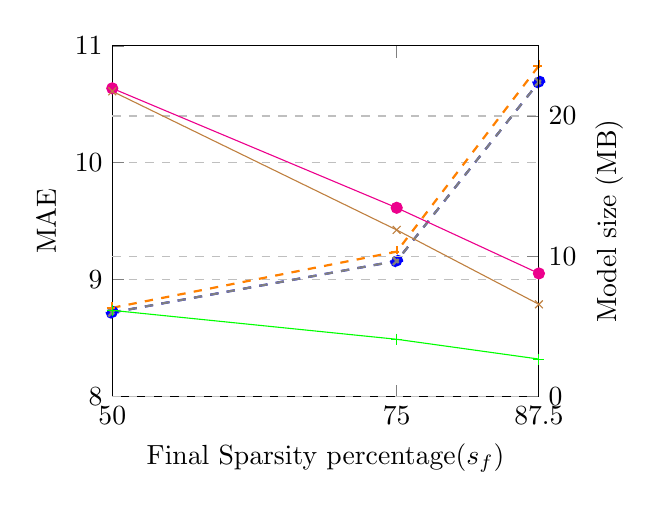
\begin{tikzpicture}

\begin{axis}[
    legend entries={Pruned model MAE,Optimized model MAE ,Quantized model MAE},
    legend to name=all_maes,
    xlabel={Final Sparsity percentage$(s{_f})$},
    ylabel={MAE},
    xmin=50, xmax=87.5,
    ymin=8, ymax=11,
    xtick={50,75,87.5,100},
    ymajorgrids=true,
    grid style=dashed,
    axis y line* = left, 
]
\addplot[
    dashed, 
    thick,
    color=blue,
        mark=*]
    coordinates {
    (50, 8.72)
    (75,9.16)
    (87.5,10.69)
    };
\addplot[
          dashed, 
    thick,
     color=gray,
        mark=x]
    coordinates {
    (50, 8.72)
    (75,9.16)
    (87.5,10.69)
    };
\addplot[
          dashed, 
    thick,
    color=orange,
        mark=+]
    coordinates {
    (50,8.76)
    (75,9.24)
    (87.5,10.83)
    };
\end{axis}

\begin{axis}[
    legend entries={Pruned model Size,Optimized model Size ,Quantified model Size},
    legend to name=sizes_alls,
    ylabel={Model size (MB)},
    xmin=50, xmax=87.5,
    ymin=0, ymax=25,
    xtick={50,75,87.5,100},
    ymajorgrids=true,
    grid style=dashed,
            hide x axis,
        axis y line*=right,
]

\addplot[
    color=magenta,
    mark=*
    ]
    coordinates {
    (50,21.97)
    (75,13.46)
    (87.5,8.78)
    };
\addplot[
    color=brown,
    mark=x
    ]
    coordinates {
    (50,21.76)
    (75,11.88)
    (87.5, 6.58)
    };
\addplot[
    color=green,
    mark=+
    ]
    coordinates {
    (50,6.15)
    (75,4.09)
    (87.5, 2.68)
    };

\end{axis}
\end{tikzpicture}

\end{document}